%% This is a tikz file
%% This template was modified from 'gecko-tree-3.tikz.tex' output by ../bin/plot-tree.py

\tikzset{node lower left/.style={font=\small,anchor=north east,text height=0.240cm,text depth=0.068cm,inner sep=0.03cm},
leaf/.style={font=\small,anchor=west,text height=0.240cm,text depth=0.068cm},
node upper left/.style={font=\small,anchor=south east,text height=0.240cm,text depth=0.068cm,inner sep=0.03cm},
bracket label/.style={font=\small,anchor=west,text height=0.240cm,text depth=0.068cm,inner sep=0.1cm},
node upper right/.style={font=\small,anchor=south west,text height=0.240cm,text depth=0.068cm,inner sep=0.03cm},
node right/.style={font=\small,anchor=west,text height=0.240cm,text depth=0.068cm,inner sep=0.03cm},
branch/.style={font=\tiny,text height=0.144cm,text depth=0.041cm,inner sep=0.025cm},
root/.style={font=\small,anchor=east,text height=0.240cm,text depth=0.068cm},
node lower right/.style={font=\small,anchor=north west,text height=0.240cm,text depth=0.068cm,inner sep=0.03cm}}

\begin{tikzpicture}[ultra thick,inner sep=0.1cm]
%  3:\hspace{15mm}\includegraphics[width=12mm,resolution=150]{../images/gekko-vittatus-1-red-shadow.png}
% +2:$T_1$
% |4:\hspace{15mm}\includegraphics[width=12mm,resolution=150]{../images/gekko-vittatus-2-orange-shadow.png}
% |
% 07:\hspace{15mm}\includegraphics[width=12mm,resolution=150]{../images/gekko-vittatus-3-yellow-shadow.png}
% 6:$T_2$
% |8:\hspace{15mm}\includegraphics[width=12mm,resolution=150]{../images/gekko-vittatus-4-green-shadow.png}
% 5
% |10:\hspace{15mm}\includegraphics[width=12mm,resolution=150]{../images/gekko-vittatus-5-blue-shadow.png}
% +9:$T_3$
%  11:\hspace{15mm}\includegraphics[width=12mm,resolution=150]{../images/gekko-vittatus-6-violet-shadow.png}

% The scale is 1.000000, and the yScale is 1.000000

%% Coordinates of nodes.
\coordinate (n0) at (0.000,3.000);
\coordinate (n1) at (0.100,3.000);
\coordinate (n1p) at (0.000,3.000);
\coordinate (n2) at (\firstdepth,4.500);
\coordinate (n2p) at (0.100,4.500);
\coordinate (n3) at (5.600,5.000);
\coordinate (n3p) at (\firstdepth,5.000);
\coordinate (n4) at (5.600,4.000);
\coordinate (n4p) at (\firstdepth,4.000);
\coordinate (n5) at (0.600,1.500);
\coordinate (n5p) at (0.100,1.500);
\coordinate (n6) at (\seconddepth,2.500);
\coordinate (n6p) at (0.600,2.500);
\coordinate (n7) at (5.600,3.000);
\coordinate (n7p) at (\seconddepth,3.000);
\coordinate (n8) at (5.600,2.000);
\coordinate (n8p) at (\seconddepth,2.000);
\coordinate (n9) at (\thirddepth,0.500);
\coordinate (n9p) at (0.600,0.500);
\coordinate (n10) at (5.600,1.000);
\coordinate (n10p) at (\thirddepth,1.000);
\coordinate (n11) at (5.600,0.000);
\coordinate (n11p) at (\thirddepth,0.000);

\coordinate (m5) at (7.5,-1.000);
\coordinate (m4) at (7.5,0.600);
\coordinate (m3) at (7.5,2.200);
\coordinate (m2) at (7.5,3.800);
\coordinate (m1) at (7.5,5.400);

\node [right=0mm of m5] {\includegraphics[height=15mm]{./pairs-3-lines-crop.pdf}};
\node [right=0mm of m4] {\includegraphics[height=15mm]{./pairs-2-3-lines-crop.pdf}};
\node [right=0mm of m3] {\includegraphics[height=15mm]{./pairs-2-2-lines-crop.pdf}};
\node [right=0mm of m2] {{\setlength{\fboxsep}{0.5mm}\setlength{\fboxrule}{1pt}\fcolorbox{pblue}{white}{\includegraphics[height=15mm]{./pairs-2-1-lines-crop.pdf}}}};
\node [right=2mm of m1] {\includegraphics[height=15mm]{./pairs-1-lines-crop.pdf}};

\node [right=19mm of m5] {\model[5]};
\node [right=19mm of m4] {\model[4]};
\node [right=19mm of m3] {\model[3]};
\node [right=19mm of m2] {\model[2]};
\node [right=19mm of m1] {\model[1]};


\coordinate (rootisland) at (\maximumdepth, -1.5);
\node [left=5mm of rootisland] {\includegraphics[width=1.2cm,angle=270,origin=c]{../island-cartoons/islands-1.pdf}};
\coordinate (tipisland) at (5.6, -1.5);
\node [right=-5mm of tipisland] {\includegraphics[width=1.2cm,angle=270,origin=c]{../island-cartoons/islands-2.pdf}};
\coordinate (island) at (\seconddepth, -1.5);
\node [right=-10mm of island] {\includegraphics[width=1.2cm,angle=270,origin=c]{../island-cartoons/islands-2.pdf}};
% \draw [->, very thick, >=stealth',\firstEventLineColor] (rootisland) -- (island);

\coordinate (ntl) at (\maximumdepth-\stemlength, -0.5);
\coordinate (ntr) at (5.6, -0.5);
\node [left=0mm of ntl] {\sffamily Time};
\draw [->, very thick, >=stealth',\firstEventLineColor] (ntl) -- (ntr);


%% maintain canvas size for pair plot
\maintainTreeCanvasSize{\draw [black!00] (n1p) -- (n1);}
\maintainTreeCanvasSize{\draw [black!00] (n2p) -- (n2);}
\maintainTreeCanvasSize{\draw [black!00] (n5p) -- (n5);}
\maintainTreeCanvasSize{\draw [black!00] (n6p) -- (n6);}
\maintainTreeCanvasSize{\draw [black!00] (n9p) -- (n9);}
\maintainTreeCanvasSize{\draw [black!00, line cap=rect] (n2p) -- (n5p);}
\maintainTreeCanvasSize{\draw [black!00, line cap=rect] (n6p) -- (n9p);}

%% events
\draw [\firstEventLineColor,very thick,dashed] (\firstdepth,-0.500) -- (\firstdepth,5.500);
\includeEventLabels{\node [text=\firstEventLabelColor,font=\LARGE,yshift=0.300cm,text height=0.415cm,text depth=0.118cm] at (\firstdepth,5.500) {\getEventLabel{\firstdepth}};}

\ifthenelse{\equal{\firstdepth}{\seconddepth}}{}{
\draw [\secondEventLineColor,very thick,dashed] (\seconddepth,-1.500) -- (\seconddepth,5.500);
\includeEventLabels{\node [text=\secondEventLabelColor,font=\LARGE,yshift=0.300cm,text height=0.415cm,text depth=0.118cm] at (\seconddepth,5.500) {\getEventLabel{\seconddepth}};}
}

\ifthenelse{\equal{\firstdepth}{\thirddepth} \OR \equal{\seconddepth}{\thirddepth}}{}{
\draw [\thirdEventLineColor,very thick,dashed] (\thirddepth,-0.500) -- (\thirddepth,5.500);
\includeEventLabels{\node [text=\thirdEventLabelColor,font=\LARGE,yshift=0.300cm,text height=0.415cm,text depth=0.118cm] at (\thirddepth,5.500) {\getEventLabel{\thirddepth}};}
}

%% horizontal lines
\ignoreForPairs{\draw (n1p) -- (n1);}
\ignoreForPairs{\draw (n2p) -- (n2);}
\draw (n3p) -- (n3);
\draw (n4p) -- (n4);
\ignoreForPairs{\draw (n5p) -- (n5);}
\ignoreForPairs{\draw (n6p) -- (n6);}
\draw (n7p) -- (n7);
\draw (n8p) -- (n8);
\ignoreForPairs{\draw (n9p) -- (n9);}
\draw (n10p) -- (n10) node[above,midway] {\small\epopsize[\descendantpopindex{1}]{}};
\draw (n11p) -- (n11) node[above,midway] {\small\epopsize[\descendantpopindex{2}]{}};

%% vertical lines
\ignoreForPairs{\draw [line cap=rect] (n2p) -- (n5p);}
\draw [line cap=rect] (n3p) -- (n4p);
\ignoreForPairs{\draw [line cap=rect] (n6p) -- (n9p);}
\draw [line cap=rect] (n7p) -- (n8p);
\draw [line cap=rect] (n10p) -- (n11p);

%% show pairs only 
\coordinate (n2m) at (\maximumdepth-\stemlength,4.500);
\coordinate (n2s) at (\firstdepth-\stemlength,4.500);
\coordinate (n6m) at (\maximumdepth-\stemlength,2.500);
\coordinate (n6s) at (\seconddepth-\stemlength,2.500);
\coordinate (n9m) at (\maximumdepth-\stemlength,0.500);
\coordinate (n9s) at (\thirddepth-\stemlength,0.500);
\includeForPairs{
    \maintainPairCanvasSize{\draw [black!00] (n2m) -- (n2);}
    % \draw (n2s) -- (n2);
    \draw (n2m) -- (n2);
    % \draw (n6s) -- (n6);
    \draw (n6m) -- (n6);
    % \draw (n9s) -- (n9);
    \draw (n9m) -- (n9) node[midway,above] {\epopsize[\rootpopindex{}]{}};
}

%% leaf labels
\node [right=0mm of n3] {
\includegraphics[width=14mm]{../phylopics/gekko-vittatus-5-teal-shadow.png}};
\node [right=0mm of n4] {
\includegraphics[width=14mm]{../phylopics/gekko-vittatus-6-auburn-shadow.png}};
\node [right=0mm of n7] {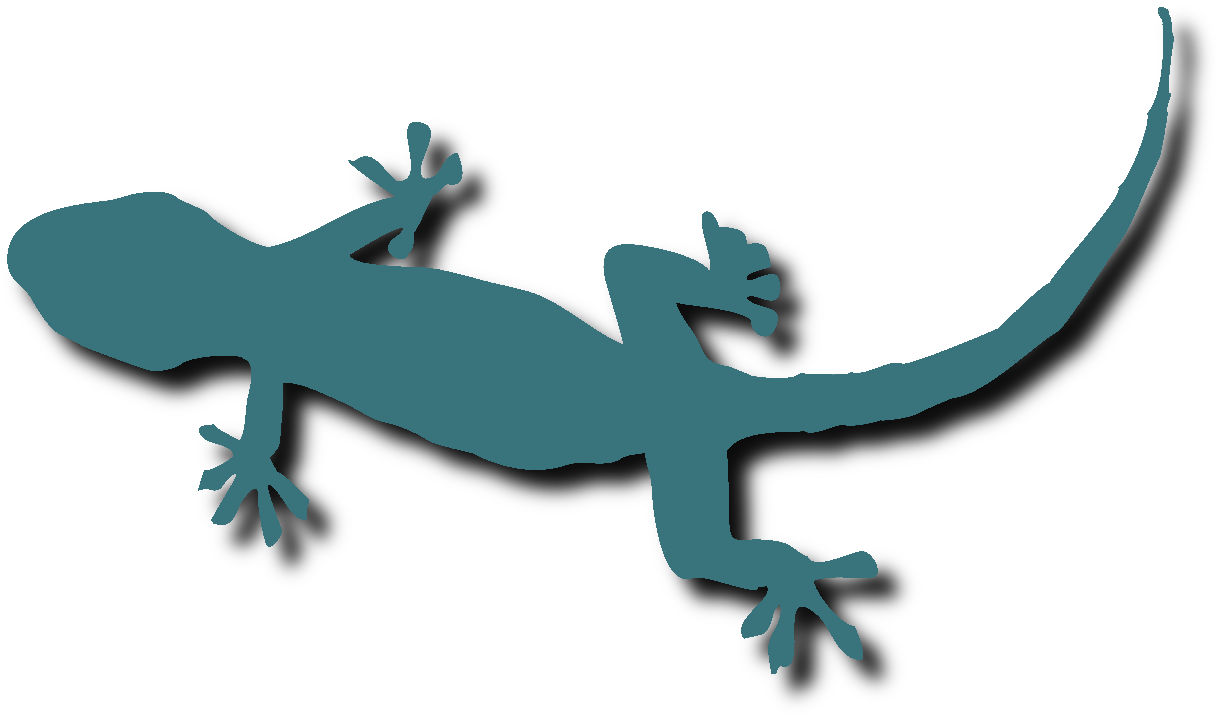
\includegraphics[width=14mm]{../phylopics/gecko-pixabay-cc0-5-teal-shadow.png}};
\node [right=0mm of n8] {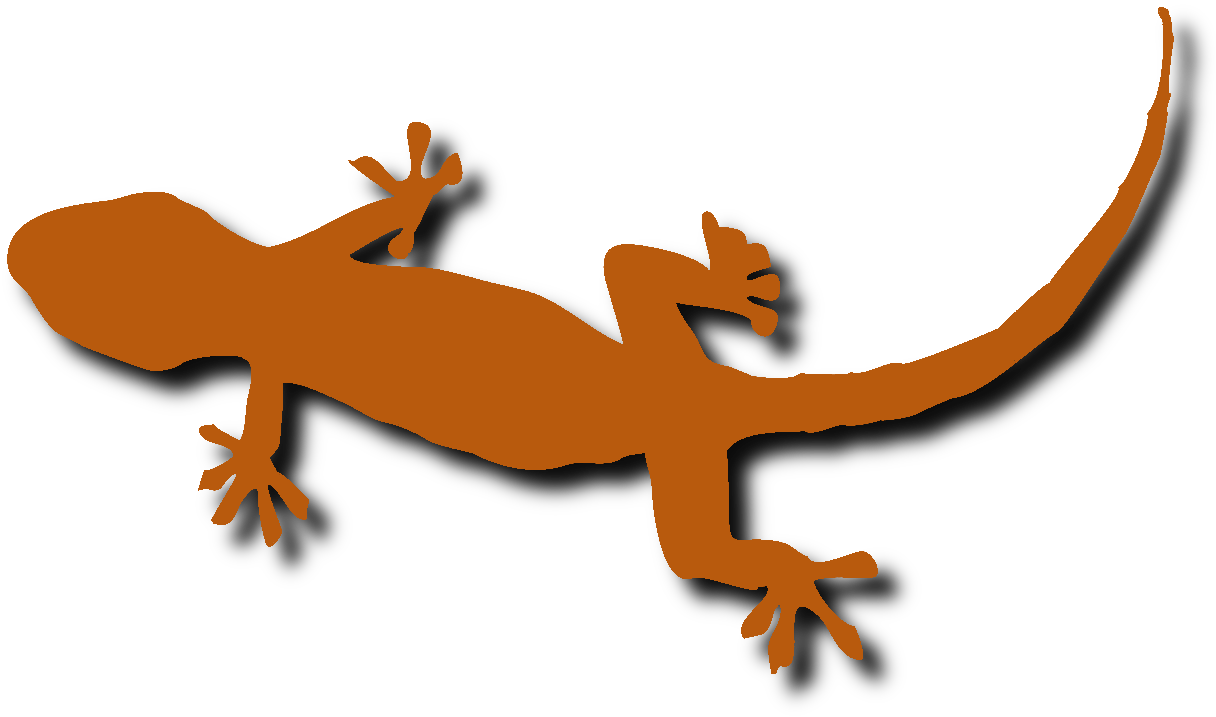
\includegraphics[width=14mm]{../phylopics/gecko-pixabay-cc0-6-auburn-shadow.png}};
\node [right=0mm of n10] {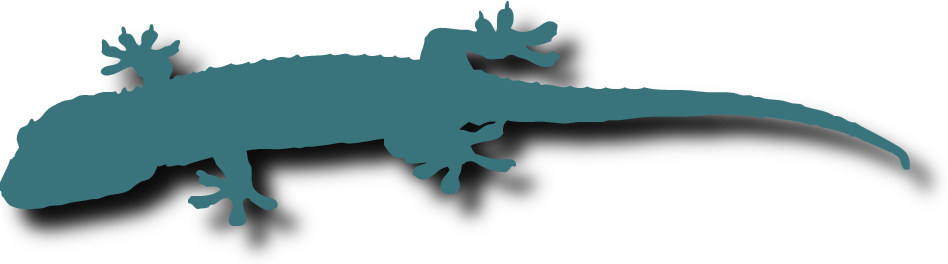
\includegraphics[width=14mm]{../phylopics/gekko-gecko-5-teal-shadow.png}};
\node [right=0mm of n11] {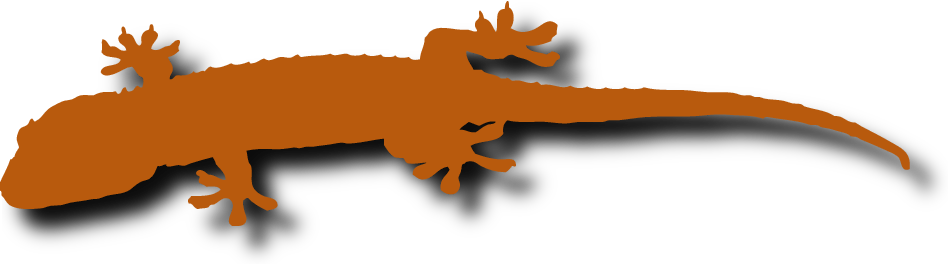
\includegraphics[width=14mm]{../phylopics/gekko-gecko-6-auburn-shadow.png}};

%% root labels
\node [left=0mm of n2m] {
\includegraphics[width=14mm]{../phylopics/gekko-vittatus-5-teal-shadow.png}};
\node [left=0mm of n6m] {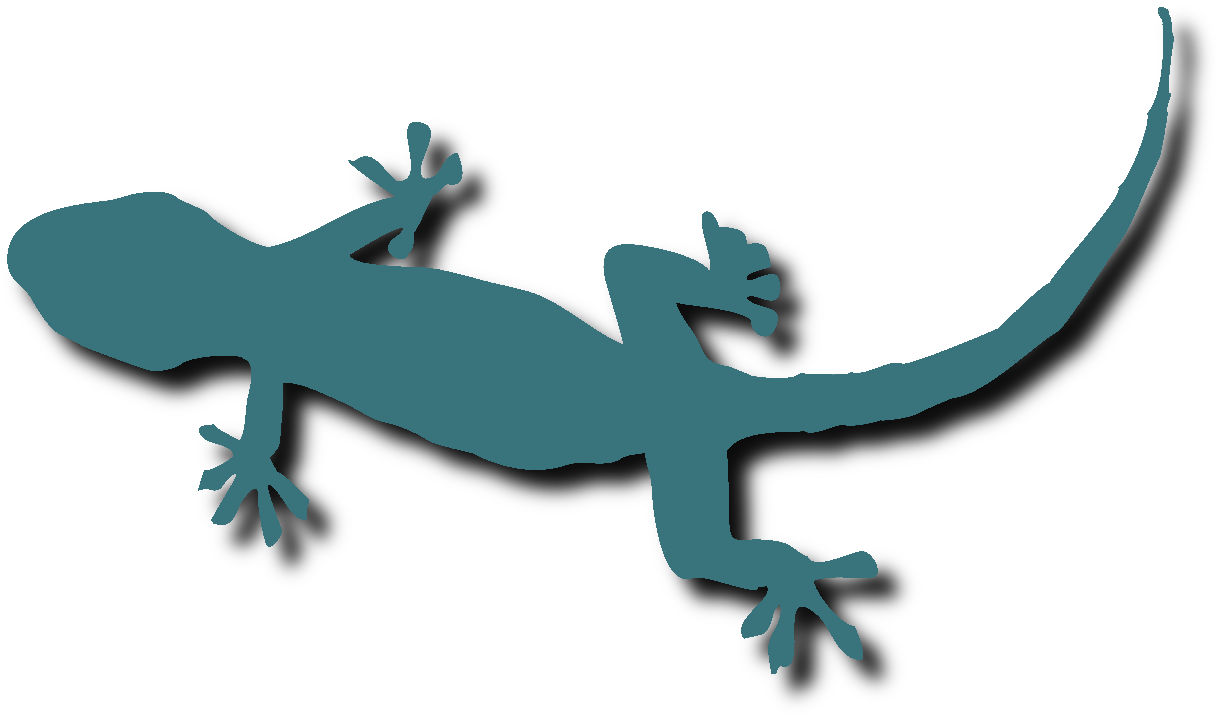
\includegraphics[width=14mm]{../phylopics/gecko-pixabay-cc0-5-teal-shadow.png}};
\node [left=0mm of n9m] {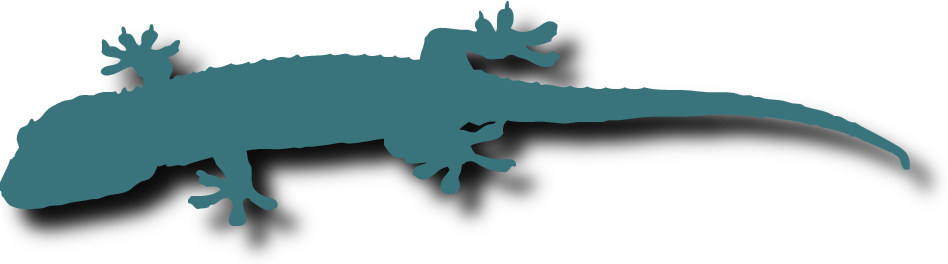
\includegraphics[width=14mm]{../phylopics/gekko-gecko-5-teal-shadow.png}};


% internal node labels (doSmartLabels is True)
\includeNodeLabels{\node [right=0mm of n2] {$\comparisondivtime{}_{\scriptscriptstyle 1}$};}
\includeNodeLabels{\node [right=0mm of n6] {$\comparisondivtime{}_{\scriptscriptstyle 2}$};}
\includeNodeLabels{\node [right=0mm of n9] {$\comparisondivtime{}_{\scriptscriptstyle 3}$};}

\end{tikzpicture}
